\documentclass{siproblemset}

\usepackage{multicol}

% SI Session Information
\course{MTH 1321}
\sessionnum{1}
\sessiondate{8/25/21}

\warmup{SI Info}
\topic{Prior Knowledge Quiz}
\topic{Review Quiz Answers}
\cooldown{Challenge Problems}

% Worksheet Information
\title{Pre-Calculus Review}
\sections{Chapter 1}
\withnamespace

\begin{document}
    \maketitle
    
    \activity{Activity 1}{Prior Knowledge Quiz}{Try these problems \textbf{alone} then compare your answers with those sitting around you.}{20 minutes}

    \begin{multipartquestion}
        \frq{What is the slope and y-intercept of $y=4-x$?.}
        \Smallsp
        \frq{What is an equation which describes the line passing through the points $(2,0)$ and $(-1,-2)$?}
        \Smallsp
    \end{multipartquestion}

    \mcq{Simplify the following expressions.}{
        \task $\dfrac{x^3-64x}{x-8}$
        \smallsp
        \task $(2^22^33^2)^{1/2}$
        \smallsp
        \task $\log_448-\log_412$
        \smallsp
        \task $2\ln5+3\ln4$
        \smallsp
        \task $8^{3\log_82}$
        \smallsp
    }

    \mcq{Simplify the following expressions.}{
        \task $\sec(u)\cos(u)$
        \smallsp
        \task $\dfrac{\tan(3x)}{\sin(3x)}$
        \smallsp
        \task $\dfrac{\cos(4x)\sin(3x)}{\cos(3x)}$
    }
    \newpage

    \frq{Fill in the following unit circle with radian angle measurements and $x$ and $y$ coordinates at the specified points.}
    \begin{tikzpicture}[scale=5.3,cap=round,>=latex, every node/.style={scale=1.3}]
    % draw the coordinates
    \draw[->] (-1.5cm,0cm) -- (1.5cm,0cm) node[right,fill=white] {$x$};
    \draw[->] (0cm,-1.5cm) -- (0cm,1.5cm) node[above,fill=white] {$y$};
    
    % draw the unit circle
    \draw[thick] (0cm,0cm) circle(1cm);
    
    \foreach \x in {0,30,...,360} {
        % lines from center to point
        \draw[gray] (0cm,0cm) -- (\x:1cm);
        % dots at each point
        \filldraw[black] (\x:1cm) circle(0.4pt);
        % draw each angle in degrees
        \draw (\x:0.6cm) node[fill=white] {$\x^\circ$};
    }

    \foreach \x in {45,135,225,315} {
        % lines from center to point
        \draw[gray] (0cm,0cm) -- (\x:1cm);
        % dots at each point
        \filldraw[black] (\x:1cm) circle(0.4pt);
        % draw each angle in degrees
        \draw (\x:0.6cm) node[fill=white] {$\x^\circ$};
    }
    
    % draw each angle in radians
    \foreach \x/\xtext in {
        30/\frac{\pi}{6},
        45/\frac{\pi}{4},
        60/\frac{\pi}{3},
        90/\frac{\pi}{2},
        120/\frac{2\pi}{3},
        135/\frac{3\pi}{4},
        150/\frac{5\pi}{6},
        180/\pi,
        210/\frac{7\pi}{6},
        225/\frac{5\pi}{4},
        240/\frac{4\pi}{3},
        270/\frac{3\pi}{2},
        300/\frac{5\pi}{3},
        315/\frac{7\pi}{4},
        330/\frac{11\pi}{6},
        360/2\pi}
    \draw (\x:0.85cm) node[fill=white] {$\hspace{.25in}$};
    
    \foreach \x/\xtext/\y in {
        % the coordinates for the first quadrant
        30/\hspace{.25in}/\hspace{.25in},
        45/\hspace{.25in}/\hspace{.25in},
        60/\hspace{.25in}/\hspace{.25in},
        % the coordinates for the second quadrant
        150/\hspace{.25in}/\hspace{.25in},
        135/\hspace{.25in}/\hspace{.25in},
        120/\hspace{.25in}/\hspace{.25in},
        % the coordinates for the third quadrant
        210/\hspace{.25in}/\hspace{.25in},
        225/\hspace{.25in}/\hspace{.25in},
        240/\hspace{.25in}/\hspace{.25in},
        % the coordinates for the fourth quadrant
        330/\hspace{.25in}/\hspace{.25in},
        315/\hspace{.25in}/\hspace{.25in},
        300/\hspace{.25in}/\hspace{.25in}}
    \draw (\x:1.25cm) node {$\left(\xtext,\y\right)$};
    
    % draw the horizontal and vertical coordinates
    % the placement is better this way
    \draw (-1.25cm,0cm) node[above=1pt] {$(\hspace{.25in},\hspace{.25in})$}
    (1.25cm,0cm)  node[above=1pt] {$(\hspace{.25in},\hspace{.25in})$}
    (0cm,-1.25cm) node[fill=white] {$(\hspace{.25in},\hspace{.25in})$}
    (0cm,1.25cm)  node[fill=white] {$(\hspace{.25in},\hspace{.25in})$};
    \end{tikzpicture}

    \mcq{Find $\theta$ such that}{
        \task $\cos \theta=\frac{\sqrt{3}}{2}$
        \Tinysp
        \task $\csc \theta=2$
    }
    \newpage
    
    \activity{Cooldown}{Challenge Problems}{Create a group of 3-4 \textbf{all with matching worksheet colors} to work on these problems together.}{10 minutes}
    
    \mcq[2]{Find the domain of the following functions. \textit{Recall that \underline{domain} refers to the set of numbers which answer the question ``What can I plug into this function?''}}{
        \task $g(t)=\sqrt{2-t}$
        \Smallsp
        \task $f(x)=\dfrac{1}{x^2}$
        \task $f(x)=x^3$
        \smallsp
    }
    
    \mcq[2]{Match the following functions with their graphs below.}{
        \task $y=mx+b$
        \smallsp
        \task $y=ax^2+b$
        \task $y=x^3$
        \smallsp
        \task $y=b^x$
        \task $y=\log_b x$
        \smallsp
        \task $y=\sqrt{x}$
    }
    \newpage
    
    \begin{multicols}{2}
        \setlength{\parindent}{0pt}
        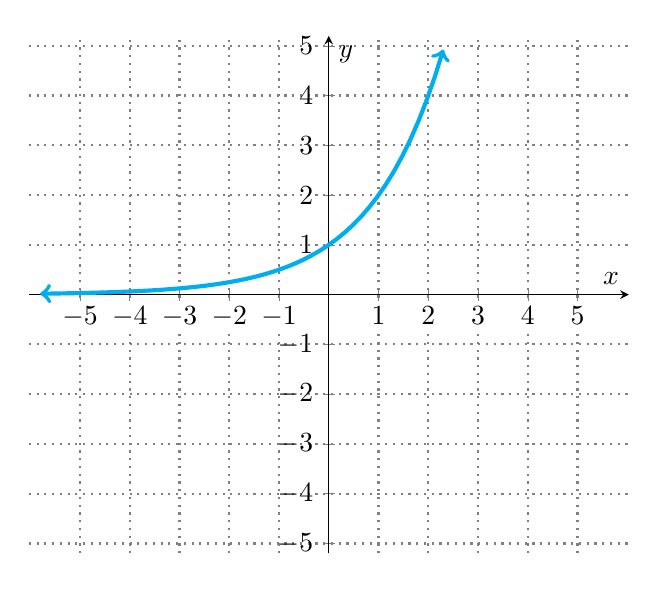
\begin{tikzpicture}
        \begin{axis}[axis x line=center, axis y line=middle,
        width=3in, %height=4in, 
        scale only axis, axis equal,
        xmin=-5.2, xmax=5.2,
        ymin=-5.2, ymax=5.2,
        xtick={-5,...,5}, ytick={-5,...,5},
        xticklabel style={draw=none, inner sep=2pt, fill=white, text opacity=1},
        xlabel={$x$}, ylabel={$y$},
        grid=both, grid style={line width=.8pt, draw=gray, dotted},
        minor tick num=0]
        \addplot[<->, cyan, line width=1.5pt, samples=50, domain=-5.8:2.3] {2^x};
        \end{axis}
        \end{tikzpicture}
        
        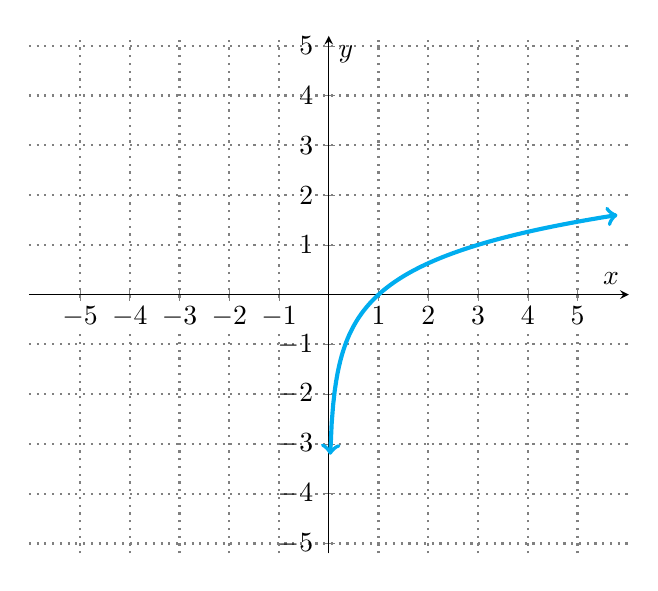
\begin{tikzpicture}
        \begin{axis}[axis x line=center, axis y line=middle,
        width=3in, %height=4in, 
        scale only axis, axis equal,
        xmin=-5.2, xmax=5.2,
        ymin=-5.2, ymax=5.2,
        xtick={-5,...,5}, ytick={-5,...,5},
        xticklabel style={draw=none, inner sep=2pt, fill=white, text opacity=1},
        xlabel={$x$}, ylabel={$y$},
        grid=both, grid style={line width=.8pt, draw=gray, dotted},
        minor tick num=0]
        \addplot[<->, cyan, line width=1.5pt, samples=200, domain=0:5.8] {ln(x)/ln(3)};
        \end{axis}
        \end{tikzpicture}
        
        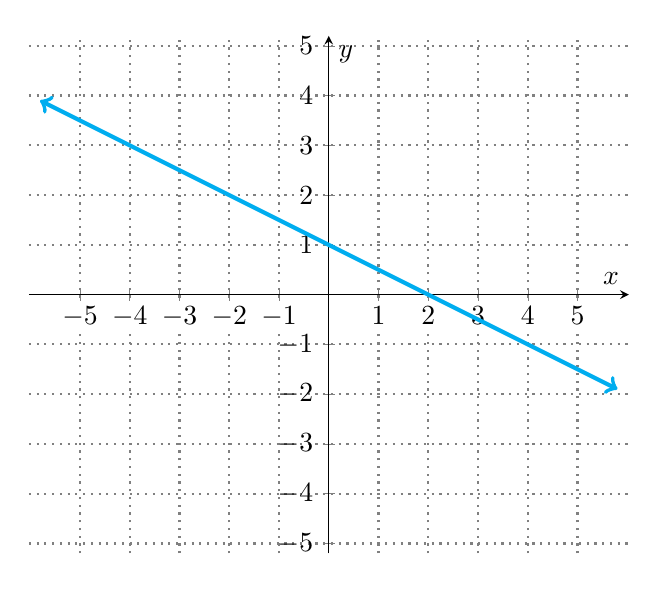
\begin{tikzpicture}
        \begin{axis}[axis x line=center, axis y line=middle,
        width=3in, %height=4in, 
        scale only axis, axis equal,
        xmin=-5.2, xmax=5.2,
        ymin=-5.2, ymax=5.2,
        xtick={-5,...,5}, ytick={-5,...,5},
        xticklabel style={draw=none, inner sep=2pt, fill=white, text opacity=1},
        xlabel={$x$}, ylabel={$y$},
        grid=both, grid style={line width=.8pt, draw=gray, dotted},
        minor tick num=0]
        \addplot[<->, cyan, line width=1.5pt, samples=50, domain=-5.8:5.8] {-1/2*x+1};
        \end{axis}
        \end{tikzpicture}
        \tinysp
        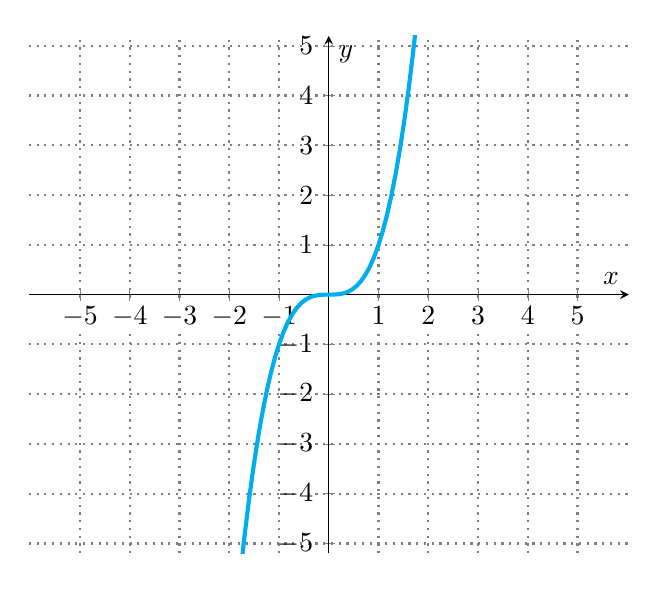
\begin{tikzpicture}
        \begin{axis}[axis x line=center, axis y line=middle,
        width=3in, %height=4in, 
        scale only axis, axis equal,
        xmin=-5.2, xmax=5.2,
        ymin=-5.2, ymax=5.2,
        xtick={-5,...,5}, ytick={-5,...,5},
        xticklabel style={draw=none, inner sep=2pt, fill=white, text opacity=1},
        xlabel={$x$}, ylabel={$y$},
        grid=both, grid style={line width=.8pt, draw=gray, dotted},
        minor tick num=0]
        \addplot[<->, cyan, line width=1.5pt, samples=50, domain=-2.12:2.12] {x^3};
        \end{axis}
        \end{tikzpicture}
        \tinysp
        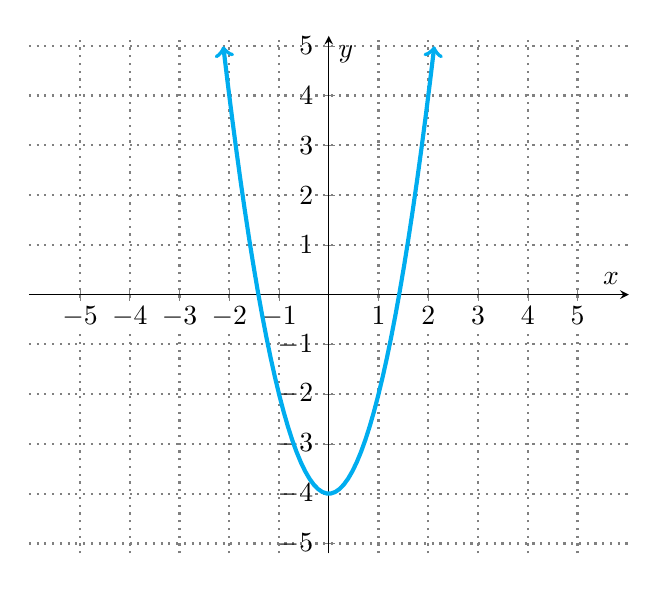
\begin{tikzpicture}
        \begin{axis}[axis x line=center, axis y line=middle,
        width=3in, %height=4in, 
        scale only axis, axis equal,
        xmin=-5.2, xmax=5.2,
        ymin=-5.2, ymax=5.2,
        xtick={-5,...,5}, ytick={-5,...,5},
        xticklabel style={draw=none, inner sep=2pt, fill=white, text opacity=1},
        xlabel={$x$}, ylabel={$y$},
        grid=both, grid style={line width=.8pt, draw=gray, dotted},
        minor tick num=0]
        \addplot[<->, cyan, line width=1.5pt, samples=50, domain=-2.12:2.12] {2*x^2-4};
        \end{axis}
        \end{tikzpicture}
        \tinysp
        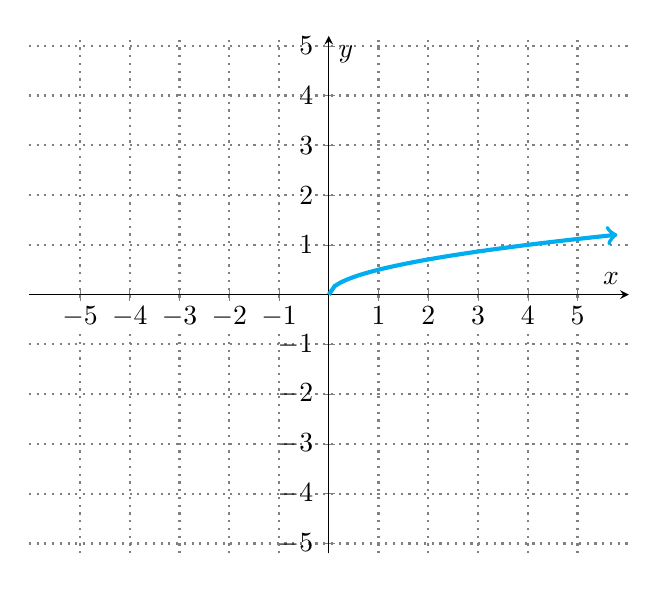
\begin{tikzpicture}
        \begin{axis}[axis x line=center, axis y line=middle,
        width=3in, %height=4in, 
        scale only axis, axis equal,
        xmin=-5.2, xmax=5.2,
        ymin=-5.2, ymax=5.2,
        xtick={-5,...,5}, ytick={-5,...,5},
        xticklabel style={draw=none, inner sep=2pt, fill=white, text opacity=1},
        xlabel={$x$}, ylabel={$y$},
        grid=both, grid style={line width=.8pt, draw=gray, dotted},
        minor tick num=0]
        \addplot[->, cyan, line width=1.5pt, samples=50, domain=0:5.8] {sqrt(x)/2};
        \end{axis}
        \end{tikzpicture}
        \tinysp
    \end{multicols}
    
\end{document}